\section{Buridan's Optimizer}
\label{sec:problems}

\begin{figure}[t]
	\centering
	\setlength{\abovecaptionskip}{0pt}
	\setlength{\belowcaptionskip}{0pt}
	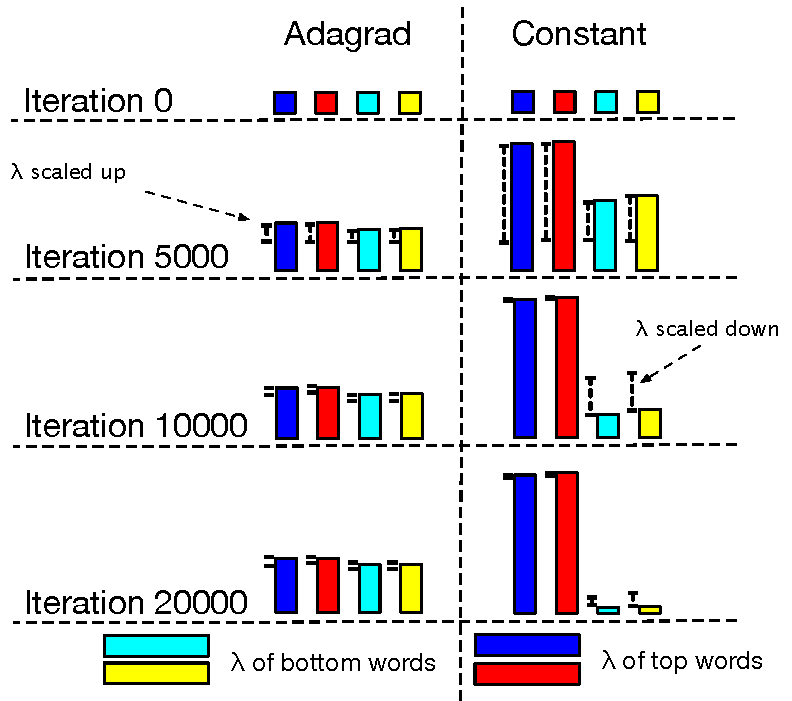
\includegraphics[width=0.45\textwidth]{2017_emnlp_adagrad_olda/figures/evolution-of-lambda.pdf}

	\caption{Illustration of \abr{adagrad}'s problem. Initially,
          the topic does not favor particular words over others, so the
          training algorithm incorrectly increases the parameters of
          bottom words. Then, \abr{adagrad} learning rates decrease too
          quickly, leaving the tie between top and bottom
          unbroken. Thus, the algorithm fails to form appropriate
          topics. A constant rate easily breaks the tie. When the tie
          is broken, the algorithm decreases the
          parameters of bottom words and increases the
          parameters of top words until convergence.}

	\label{fig:lambda_evolution_catroon}      
\end{figure}

Latent Dirichlet allocation~\cite[\abr{lda}]{blei2003latent} is
perhaps the most well known topic model.  In this section, we analyze
problems with \adagrad{} for online
\abr{lda}~\cite{hoffman2010online}, and provide some solutions. Our
analysis is easy to generalize to other online topic models, e.g.,
online Hierarchical Dirichlet
Process~\cite[\abr{hdp}]{wang2011online}.

\subsection{Online \abr{lda}}

To train \abr{lda}, we want to compute the posterior
\begin{align*}
	p(\beta,\theta, & z \g w, \alpha, \eta) \propto \prod_{k=1}^{K}p(\beta_k \g \eta) \cdot \\
	&\prod_{d=1}^{D}p(\theta_d \g \alpha)\prod_{n=1}^{N_d}p(z_{dn} \g \theta_d)p(w_{dn} \g \beta_{z_{dn}}),
\end{align*}
where $\beta_k$ is the topic-word distribution for the $k^\text{th}$ of $K$ topics,
$\theta_d$ is the document-topic distribution for the $d^\text{th}$ of $D$ document,
$z_{dn}$ is the topic assignment for the $n^\text{th}$ of $N_d$ words in in the $d^\text{th}$ document,
$w_{dn}$ is the word type of the $n^\text{th}$ word in the $d^\text{th}$ document,
with $\alpha$ and $\eta$ the Dirichlet priors over the document-topic and
topic-word distributions.

However, this is intractable. Stochastic variational inference
(\abr{svi}) is a popular approach for approximation. It first posits a
mean field variational distribution
\begin{align*}
	q(\beta, \theta, z \g & \lambda, \gamma, \phi) = \prod_{k=1}^{K}q(\beta_k \g \lambda_k) \cdot \\
	& \prod_{d=1}^{D}q(\theta_d \g \gamma_d)\prod_{n=1}^{N_d}q(z_{dn} \g \phi_{dn}),
\end{align*}
where $\gamma$
(Dirichlet) and $\phi$ (multinomial) are local parameters and $\lambda$
(Dirichlet) is a global parameter.
\abr{svi} then optimizes the variational parameters to minimize the
\abr{kl} divergence between the variational distribution and the true
posterior.


At iteration $t$, \abr{svi} samples a document $d$ from the corpus and
updates the local parameters:
\begin{align}
	\phi _{vk}^{d} & \propto \ex{ \digam {\gamma _{dk}} + \digam
                         {\lambda _{kv}^{(t)}} - \digam {\sum\limits_i
                         {\lambda _{ki}^{(t)}} }},
\label{eq: update_phi} \\
\gamma _k^{d} & = \alpha  + \sum\limits_v {{n_v}\phi _{vk}^{d}},
\end{align}
where $n_v$ is the number of words $v$ in $d$, and $\digam{.}$ is the
digamma function. After finding $\phi^d$ and $\gamma^d$,
\abr{svi} optimizes the global parameters using stochastic gradient
ascent,

\begin{eqnarray}
\lambda _{kv}^{(t + 1)} &=& (1 - \rho _{kv}^{(t)})\lambda _{kv}^{(t)} + \rho _{kv}^{(t)}(\eta  + D\phi _{vk}^d{n_{dv}}) \nonumber\\
&=& (1 - \rho _{kv}^{(t)})\lambda _{kv}^{(t)} + \rho _{kv}^{(t)}\hat \lambda _{kv}^{(t)} \nonumber\\
&=& \lambda _{kv}^{(t)} + \rho _{kv}^{(t)}g_{kv}^{(t)},
\label{eq : update_lambda}
\end{eqnarray}
where $\rho^{(t)}$ is the learning rate, $\hat \lambda _{kv}^{(t)} = \eta + D{\phi^{d} _{vk}}{n_{dv}}$ is the intermediate parameter and $g_{kv}^{(t)} =  - \lambda _{kv}^{(t)} + \hat \lambda _{kv}^{(t)}$ is the gradient.




\subsection{\abr{adagrad} for Online \abr{lda}}

In general, $\rho_{kv}^{(t)} = \kappa^{(t)}$, for all $v \in {1,..,V}$ and $k
\in {1,...,K}$, where $\kappa^{(t)}$ can be a decreasing rate~\cite{hoffman2013stochastic}, a small constant~\cite{collobert2011natural} or an adaptive
rate~\cite{ranganath2013adaptive}. These three methods are all global learning
rate methods, which cannot adaptively adjust learning rate for each dimension
of the parameter, or address the problems caused by sparse gradients.

\abr{adagrad} is a popular learning rate method designed for online
optimization problems with high dimension and sparse gradients. Thus, it seems
reasonable to apply \abr{adagrad} to update learning rates for online topic
models. When using \abr{adagrad} \cite{duchi2011adaptive} with online
\abr{lda}, the update rule for the each learning rate is

\begin{equation}
\rho_{kv}^{(t)} = \frac{\rho_0}{\sqrt{\epsilon + \sum_{i=0}^{t}\left( g_{kv}^{(i)} \right)^2}},
\end{equation}
where $\rho_0$ is a constant, and a very small $\epsilon$ guarantees that the learning rates are non-zero.

\subsection{\abr{adagrad}'s Indecision}

A philosophical thought experiment provides us with the story of Buridan's
ass~\cite{bayle-1826}: situated between two piles of equally tasty hay, the
poor animal starved to death.  \abr{adagrad} faces a similar problem in
breaking the symmetries of common variational inference initializations. For
convenience, we unfold an example with a single document at each iteration. Our
analysis generalizes to mini-batches.

Initially, the topics $\beta_{1:K}$ do not favor particular words over
others as inference cannot know \textit{a priori} which words will have high
probability in a particular topic.
The algorithm must break ties between parameters of the top and
bottom words in a topic.
Unfortunately, the momentum of \abr{adagrad} fails for topic models.
We now explain why this is.

\abr{adagrad} looks to the gradient for clues about what features will
be important.  This is because before the equilibrium is
broken, the values of different
$\lambda_{kv}$ are close, so Equation \ref{eq: update_phi} will be
approximately seen as $\phi_{vk}^d \propto \ex{\digam{\gamma_{dk}}}$, which
implies that $\lambda$ has very small influence on the optimization of
$\phi$.
If some topics are prevalent in the sampled document~$d$, large probability
will be assigned to the corresponding $\phi_{.k}$, meaning that all words
in document $d$ are treated as top words.  The initial clues are at
best random and at worst counter productive.

However, \abr{adagrad} uses these cues to prefer some dimensions over
others.  Let $\lambda^*$ be the optimum; the topic \abr{adagrad} should find at
convergence: $\lambda^*_{kv} \approx \e{}{\hat \lambda^{(t)}_{kv}}$. By definition, once the algorithm
converges, $\lambda^*_{kv}$ for top words will have very large
values while $\lambda^*_{kv}$ for bottom words will be small.  After
using noisy momentum terms, it must overcome initial faulty signals.


We now show the lower and upper bounds of
$\e{}{\hat\lambda^{(t)}_{kv}}$ to show how big of an uphill battle
\abr{adagrad} faces. Expanding the update rule,
\begin{eqnarray*}
	\e{}{\hat \lambda^{(t)}_{kv}} &=& \e{}{\eta + D{\phi^{d} _{vk}}{n_{dv}}} \\
	&=& \eta + D\bar{n}_v\e{}{\phi_{vk}}, \\
\end{eqnarray*}
where $\bar{n}_v = \sum_{i=1}^{D}n_{iv}/D$. By definition, $\phi_{vk}$ is the probability
that word $v$ is assigned to topic $k$. 
Thus after convergence, for a bottom word, $\phi_{vk} \to 0$, and $\e{}{\phi_{vk}} \approx \eta$. For a top word, $\phi_{vk} \ge 1 / K$, $1/ K \le \e{}{\phi_{vk}} \le 1$, and
the lower and upper bounds of $\e{}{\hat\lambda^{(t)}_{kv}}$ are
\begin{equation*}
	\eta + (1/ K)D\bar{n}_v \le	\e{}{\hat \lambda^{(t)}_{kv}} \le \eta + D\bar{n}_v.
\end{equation*}
The size of the dataset determines $D\bar{n}_v$.
Thus for top words, $\lambda^*_{kv}$ will converge to a large value:
quite a large hill to climb. 

\abr{adagrad} uses the accumulations of previous gradients as learning
rates' denominators. Thus, how quickly the algorithm climbs the hill is inversely proportional to
the gradient size. We next show that the magnitude of gradients of top words are very large before
the algorithm converges. Let $g^*$ be the gradient after convergence. We show
the bounds of $|g_{kv}|$, where $|.|$ is the absolute value, in the following:
\begin{eqnarray*}
	\g g_{kv}^{*} \g &=& \g - \lambda _{kv}^* + \eta  + D\phi _{vk}^d{n_{dv}} \g\\
	&\approx& \g - \eta  - D\bar{n}_vE[{\phi _{vk}}] + \eta  + D\phi _{vk}^d{n_{dv}} \g \\
	&\approx& \e{}{\phi_{vk}}*D \g n_{dv} - \bar{n}_v \g.
\end{eqnarray*}
Thus,
\begin{equation*}
     (D/K) \g n_{dv} - \bar{n}_v \g \le	\g g_{kv}^{*} \g  \le D \g n_{dv} - \bar{n}_v \g.
\end{equation*}
Only when $n_{dv} = \bar{n}_v$, does $\g g_{kv}^{(t)} \g = 0$.
Otherwise, due to the large $D$, $\g g_{kv}^{*} \g$ will be large. However,
in practice, $n_{dv}$ varies largely from document to document, which leads
to large values of $\g g_{kv}^{*} \g$.
Based on this property of the gradient, when $\lambda_{kv}$ is far away from the
optimum, $\g g^{(t)}_{kv} \g \ge \g g^*_{kv} \g$.
Thus, the values of $\g g^{(t)}_{kv} \g$ for top words are very large before
convergence.

Because of these large gradients in the first
several iterations, learning rates soon decrease to small values; even
if a topic has gathered a few words, \adagrad{} lacks the momentum to
move other words into the topic. These small learning rates slow the
updates of $\lambda$.

In sum, the initial gradient signals confuse the algorithm, the
gradients are large enough to impede progress later, and large datasets
imply a very large hill the algorithm must climb.  Since the update
progresses slowly, online \abr{lda} needs more iterations to break the
equilibrium. Because the gradients of all words are still very large,
the learning rates decrease quickly, which makes the update progress
more slowly.
When the update progresses more slowly, online \abr{lda} needs
more iterations to break the tie. This cycle repeats, until some
learning rates decrease to zero and learning effectively stops. Thus, the
algorithm will never break the tie or infer good
topics. Figure~\ref{fig:lambda_evolution_catroon} illustrates the
problem of online \abr{lda} with \abr{adagrad}.

\subsection{Alternative Solutions}



\abr{adadelta}~\cite{zeiler2012adadelta} and \abr{adam}~\cite{kingma2014adam}
are extensions to \abr{adagrad}.
\abr{adadelta} does not have guaranteed convergence on convex optimization
problems. Even though \abr{adam} has a theoretical bound on its convergence
rate, it is controlled by and sensitive to several learning rate parameters.
For good performance with \abr{adam}, manual adjustment is necessary.
In addition, since \abr{adadelta} computes the moving average of updates, and
\abr{adam} needs to compute the bias-corrected gradient estimate, they require
more intricate implementations. Consequently, these two methods are not as popular as \abr{adagrad} for beginners. However, for \abr{svi} latent variable models, they can address the problems with \abr{adagrad}.



\abr{adadelta} updates the learning rates with the
following rule:
\begin{equation}
\rho _{kv}^{(t)} = \frac{{\sqrt {\e{}{(\lambda _{kv}^{(t)} - \lambda _{kv}^{(t - 1)})} + \varepsilon } }}{{\sqrt {\e{}{g_{kv}^{(t)}} + \varepsilon } }},
\end{equation}
where $\e{}{x^{(t)}}= {\rho _0}\e{}{x^{(t - 1)}} + (1 - {\rho _0}){({x^{(t)}})^2}$, $\rho_0$ is a decay constant, and  $\varepsilon$ is for numerical stability.

\abr{adam}'s update rule is determined based on estimates of first and
second moments of the gradients:
\begin{eqnarray}
&&m_{kv}^{(t)} = {b_m}m_{kv}^{(t - 1)} + (1 - {b_m})g_{kv}^{(t)}, \nonumber\\
&&u_{kv}^{(t)} = {b_u}u_{kv}^{(t - 1)} + (1 - {b_u}){(g_{kv}^{(t)})^2}, \nonumber\\
&&\hat m_{kv}^{(t)} = \frac{{m_{kv}^{(t)}}}{{1 - b_m^t}}, \hat u_{kv}^{(t)} = \frac{{u_{kv}^{(t)}}}{{1 - b_u^t}}, \nonumber\\
&&\lambda _{kv}^{(t + 1)} = \lambda _{kv}^{(t)} + {\rho _0}\hat m_{kv}^{(t)}/(\sqrt {\hat u_{kv}^{(t)}}  + \varepsilon )
\label{eq: adam_update_rule},
\end{eqnarray}
where $\rho_0$ is a constant, $b$ controls the decay rate.



Both \abr{adadelta} and \abr{adam} use the moving average of gradients as the
denominator of learning rates. The learning rates will not monotonically
decrease, but vary in a certain range. This property prevents online topic
models from being trapped and
breaks the tie between top words and bottom topic words.
\abr{adam} in particular uses bias-corrected estimate of gradient $\hat
m_{kv}$, rather than the original stochastic gradient $g_{kv}$ to guide
direction for the optimization and therefore achieves better results.

In addition, the magnitude of gradients is proportional to the
dataset's size. Thus, when the dataset is small enough, \abr{adagrad}
will still work.
